{\sl This fieldstone was developed in collaboration with L. van de Wiel}. 


The following problem is studied in \cite{jolm17}. The equations that they solve are the following ones:

The equation to solve are:
\begin{eqnarray}
-\vec{\nabla}p + \Delta \vec{\upnu} + Ra T \vec{e}_y &=& 0\\
\vec\nabla\cdot\vec\upnu &=& 0 \\
-\Delta T + \vec\upnu\cdot\nabla T &=& 0
\end{eqnarray}

The domain is chosen to be the right triangle
with vertices $(0,0)$, $(1,0)$, and $(0,1)$. 
The boundary is considered to be solid walls (no-slip).
For the temperature, a sinusoidal heat source is enforced on the bottom
boundary with a Dirichlet condition ($T(x)=2(1-\cos (2\pi x))$), 
the left wall is set to a constant temperature
of zero, and the hypotenuse wall is perfectly insulated so that a Neumann 
boundary condition is appropriate.

The steady state velocity pressure and temperature fields as shown in 
\cite{jolm17} are as follows:

\begin{center}
a)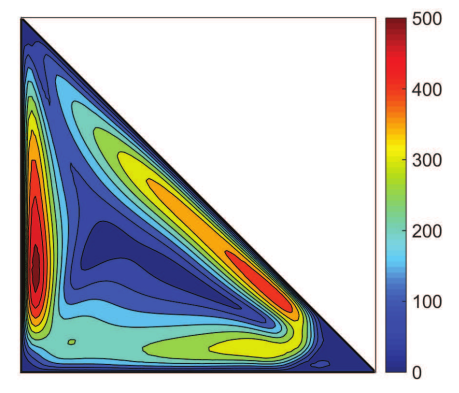
\includegraphics[width=4.5cm]{python_codes/fieldstone_51/images/jolm17_vel}
b)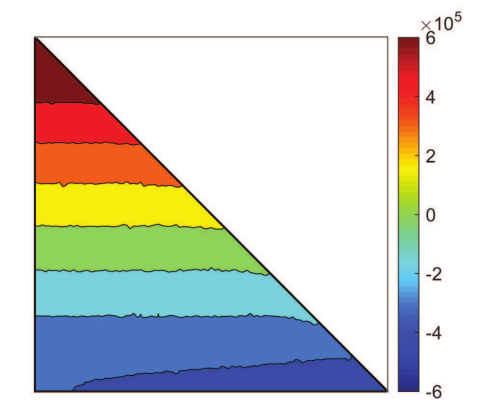
\includegraphics[width=4.5cm]{python_codes/fieldstone_51/images/jolm17_p}
c)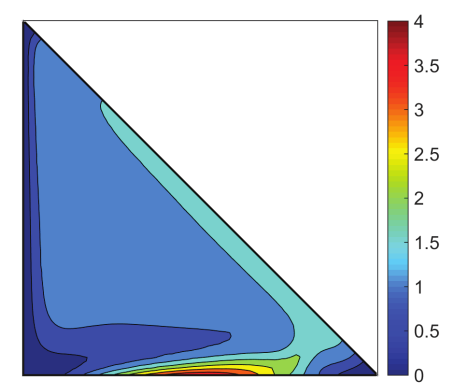
\includegraphics[width=4.5cm]{python_codes/fieldstone_51/images/jolm17_T}\\
{\small Steady state fields: a) velocity, b) pressure, c) temperature.}
\end{center}

Although it is not mentioned in the original article it appears that the 
pressure field has been normalised so that $\langle p \rangle = \int_\Omega p dV=0$.

As opposed to the mesh presented in \cite{jolm17} we build a regular mesh.
An example of such a mesh is shown hereunder for $n=5$ (the number of nodes
per side of the triangular domain). 
\begin{center}
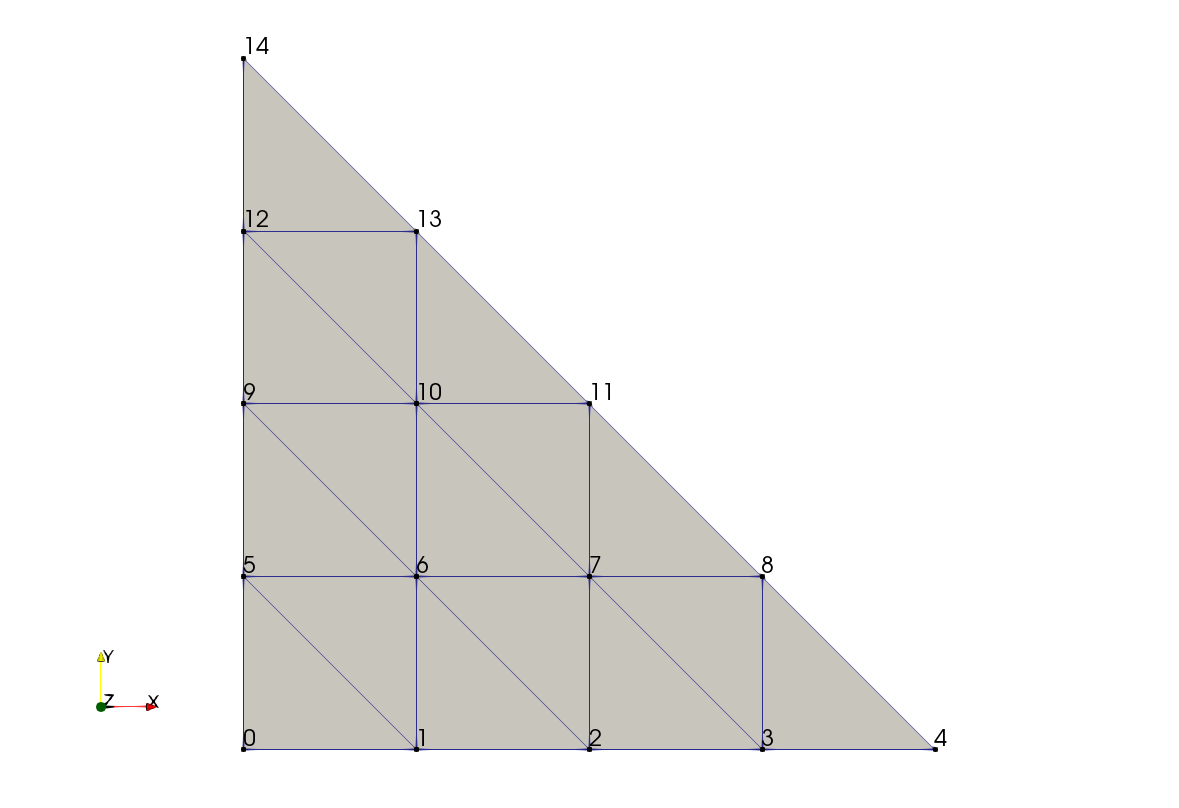
\includegraphics[width=6cm]{python_codes/fieldstone_51/images/minigrid5}
\end{center}

Instead of the steady-state equations above we solve the time-dependent 
heat transport equation with $k=1$, $C_p=1$ and $\rho_0=1$. At steady state 
we will have $\partial T/\partial t=0$ and our equation will become identical 
to theirs. 

Additionally we measure:
\begin{itemize}
\item the Nusselt number defined by 
\[
Nu
=\int_{y=0} \vec{\nabla}T \cdot \vec{n} dS  
=-\int_{x=0}^{x=1} \frac{\partial T}{\partial y} dx 
\]
It is reported to be 24.535 in \cite{jolm17}.
\item the temperature on the hypotenuse.
\item the root mean square velocity
\item the mean temperature $\langle T \rangle = |\Omega|^{-1} \int_\Omega T \; dV$
\end{itemize}

\begin{center}
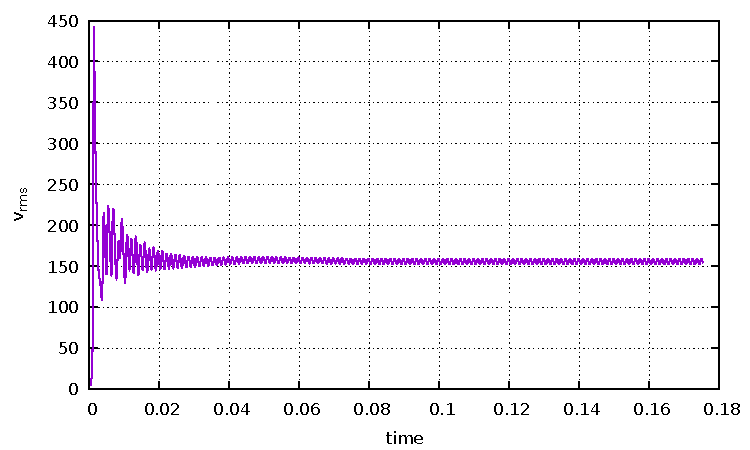
\includegraphics[width=6cm]{python_codes/fieldstone_51/images/vrms.pdf}
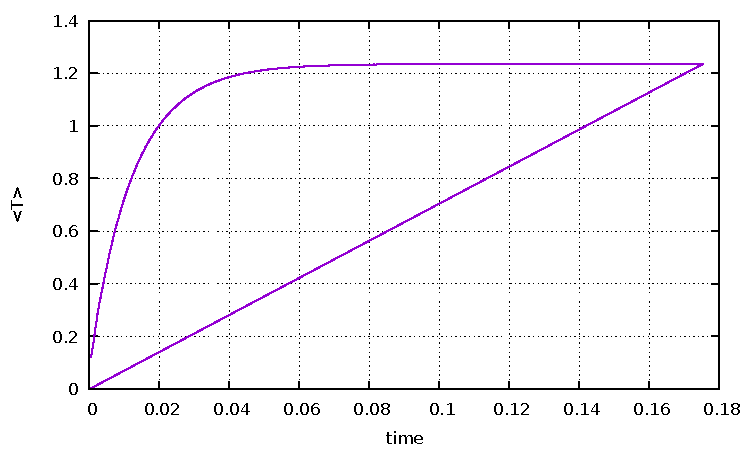
\includegraphics[width=6cm]{python_codes/fieldstone_51/images/avrgT.pdf}\\
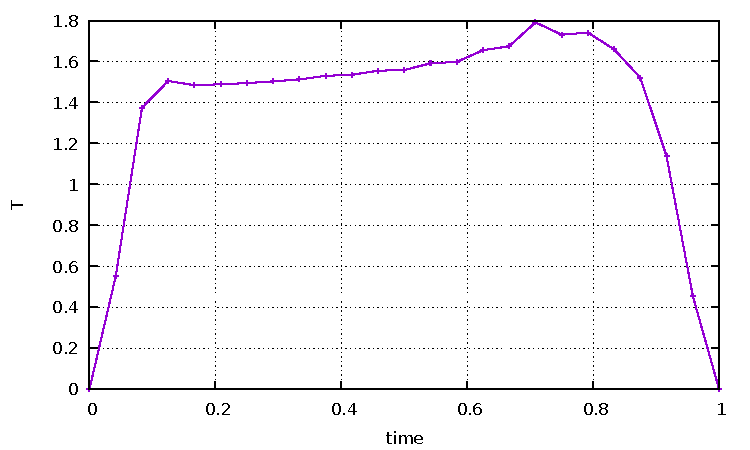
\includegraphics[width=6cm]{python_codes/fieldstone_51/images/temp_hyptenuse.pdf}
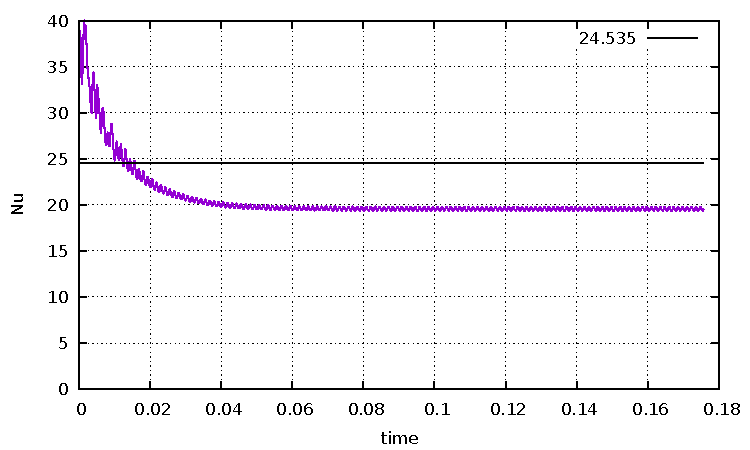
\includegraphics[width=6cm]{python_codes/fieldstone_51/images/Nu.pdf}
\end{center}

\begin{center}
a)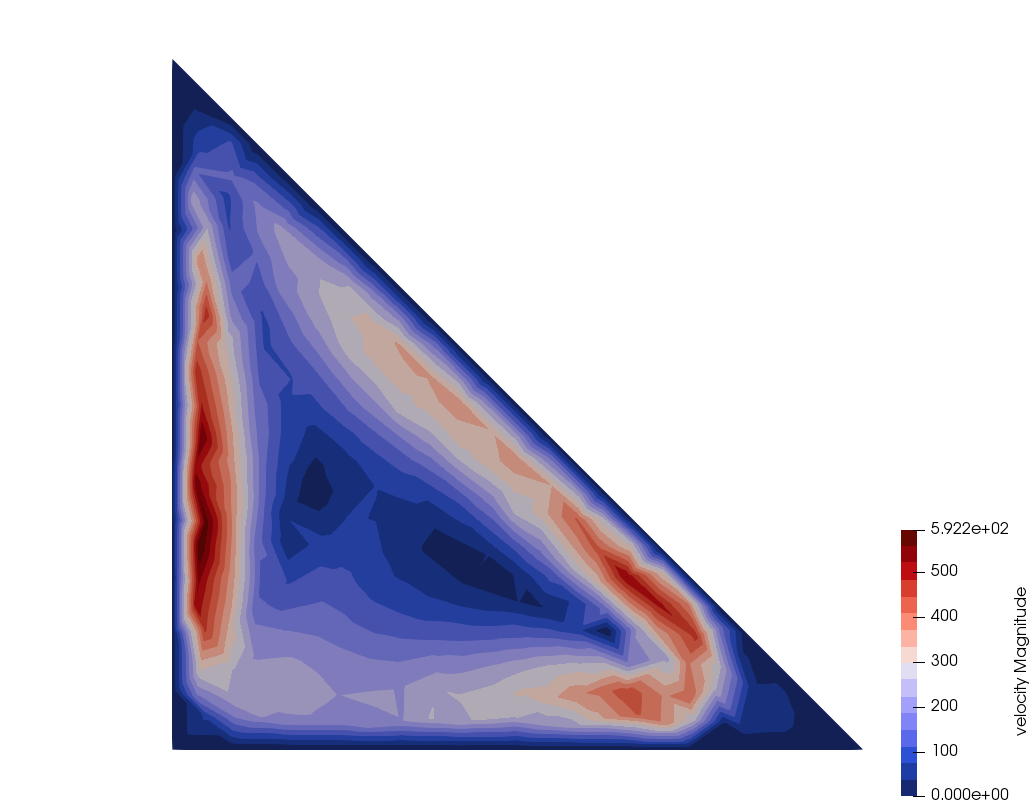
\includegraphics[width=4.5cm]{python_codes/fieldstone_51/images/vel}
b)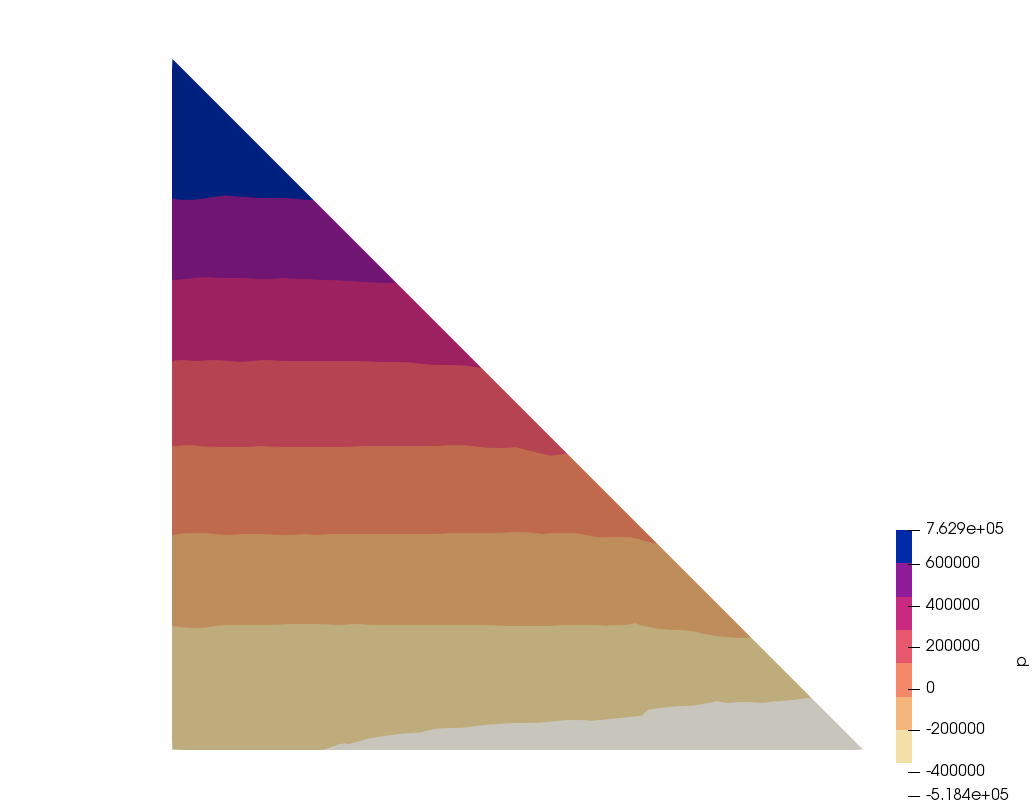
\includegraphics[width=4.5cm]{python_codes/fieldstone_51/images/press}
c)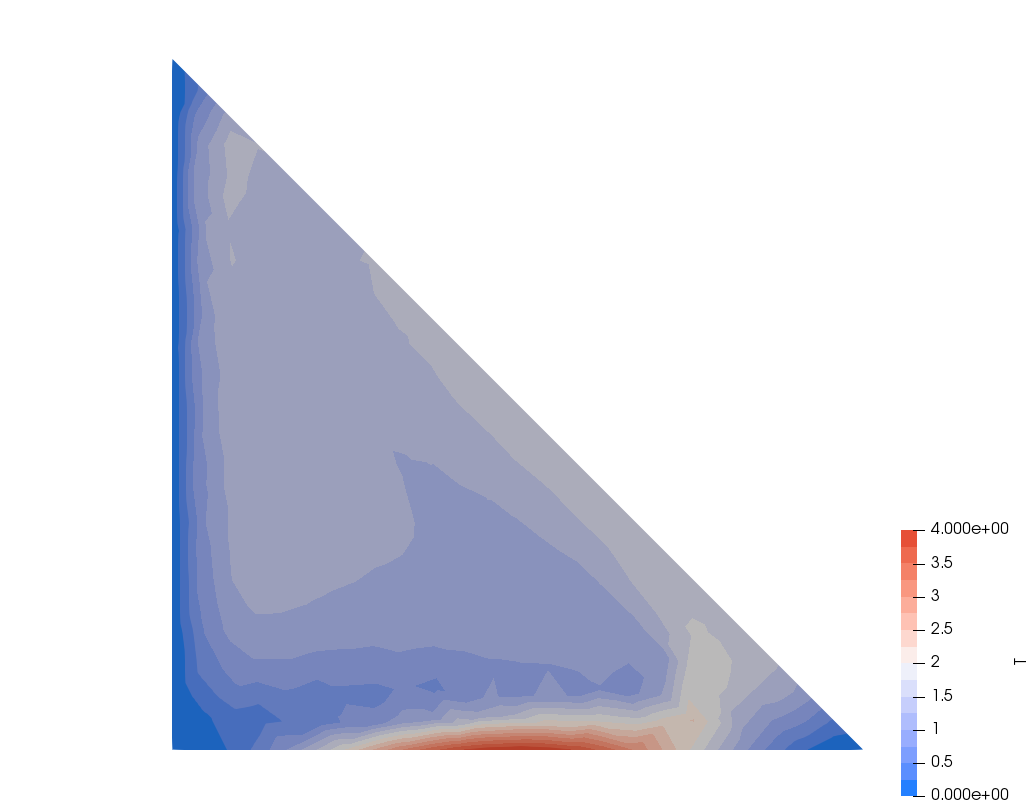
\includegraphics[width=4.5cm]{python_codes/fieldstone_51/images/temp}\\
{\small Steady state fields: a) velocity, b) pressure, c) temperature.}
\end{center}




